\section{Preliminaries}

In this work, we describe a full pipeline using MNE to analyze the OpenfMRI dataset ds000117 by~\cite{wakeman2015multi}. The data consist of simultaneous M/EEG recordings from 19 healthy participants performing a visual recognition task. Subjects were presented images of famous, unfamiliar and scrambled faces. The dataset provides a rich context to study different neuroscientific and cognitive questions, such as: Which brain dynamics are characteristic of recognizing familiar as compared to unfamiliar faces? How do commonly studied face-responsive brain regions such as the \ac{STS}, the \ac{FFA} and the \ac{OFA} interact when processing the familiarity of the face? At the same time, it presents a well-studied paradigm which can be particularly beneficial for the development of methods related to connectivity and source localization.

\subsection{Data description}

The subjects participated in 6 runs, each 7.5 minutes in duration. In the original study, three subjects were discarded due to excessive artifacts in the data. To produce comparable results, the same subjects are also discarded from the group results in this study. The data were acquired with an Elekta Neuromag Vectorview 306 system consisting of 102 magnetometers and 204 planar gradiometers. In addition, a 70 channel Easycap EEG system was used for recording EEG data simultaneously.

\subsection{Reading data}
MNE supports multiple file formats written by M/EEG hardware vendors.
Apart from Neuromag \textit{FIF} files, which are the default storage format, MNE can natively read multiple other formats ranging for MEG data including 4D Neuroimaging BTI, KIT, and CTF, and for EEG data B/EDF, EGI, and EEGLAB \textit{set}\footnote{\url{http://martinos.org/mne/stable/manual/io.html}}. Despite this heterogeneity of systems, MNE offers a coherent interface to the metadata of the recordings using the so-called \emph{measurement info}\footnote{\url{http://martinos.org/mne/stable/auto_tutorials/plot_info.html}}.
Regardless of the input format, all processed files can be saved as \textit{FIF} files or in the HDF5 format\footnote{\url{https://support.hdfgroup.org/HDF5/}}.

MNE can handle multimodal data containing different channel types, the most common being magnetometer, gradiometer, \ac{EEG}, \ac{EOG}, \ac{ECG}, and stimulus trigger channels that encode the stimulation paradigm. MNE also supports \ac{EMG}, stereotactic EEG (sEEG) and electrocorticography (ECoG), \ac{fNIRS} or miscellaneous (misc) channel types. Declaring and renaming channel types is a common step in the preparation of M/EEG datasets before analysis. In our case, once the files were read in, some of the channels needed to be renamed and their channel types corrected in the measurement info (see~\citep{wakeman2015multi}): the EEG061 and EEG062 electrodes were set as EOG, EEG063 was set as ECG, and EEG064 was set as a miscellaneous channel type as it was a free-floating electrode. If this step is omitted, some preprocessing functions may fall back to potentially less optimal defaults, for example, using the average of the magnetometers instead of the ECG channel when searching for cardiac events.

\section{MEG and EEG data preprocessing}

\subsection{Maxwell filtering (SSS)}
\label{sec:maxfilter}

\begin{figure}[htb]
        \centering
        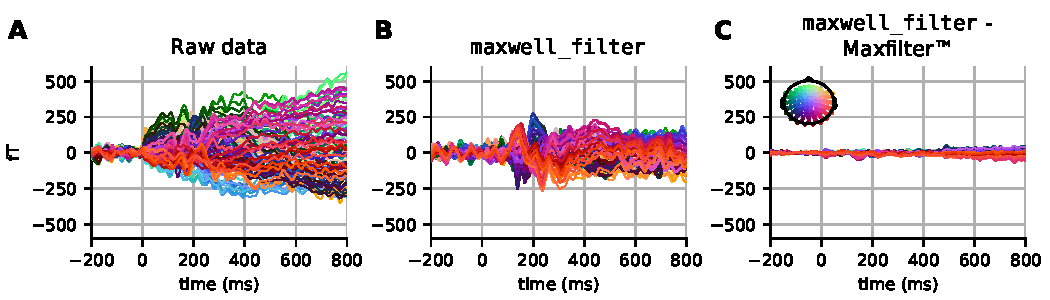
\includegraphics[width=\linewidth]{figures/Maxfilter.pdf}
        \caption[Comparison of Elekta MaxFilter (TM) and MNE implementation]{Evoked responses (filtered between 1 and 40 Hz) in the magnetometer channels from (A) unprocessed data, (B) data processed with \code{maxwell\_filter} in MNE, and (C) the difference between data processed using \code{maxwell\_filter} and Elekta MaxFilter (TM). The colors show the sensor position, with $(x, y, z)$ sensor coordinates converted to $(R, G, B)$ values, respectively.}
        \label{fig:fig_maxwell}
\end{figure}

% mj: you can also have artifacts inside the room
% In the absence of an excellent magnetically shielded room or a very quiet electromagnetic environment
Neuromag MEG recordings are often preprocessed first using the Signal Space Separation (SSS) method~\citep{taulu2006spatiotemporal}, otherwise known as Maxwell filtering. SSS decomposes the data using multipole moments based on spherical harmonics and removes the component of magnetic field originating from outside the MEG helmet. SSS is therefore useful for removing environmental artifacts, and can also be used to compensate for head movements during the recording. In this study, movement compensation is not strictly necessary as the participants managed to stay predominantly still.

The data provided by OpenfMRI~\citep{poldrack2017openfmri} already contain files processed using the proprietary Elekta software MaxFilter, which is what we use in our analysis for the sake of reproducibility. However, MNE offers an open source reimplementation and extension of SSS as well. Before running SSS, it is crucial that bad channels are marked, as otherwise SSS may spread the artifacts from the bad channels to all other MEG channels in the data. This step is preferably done manually with visual inspection. When using the MNE implementation of Maxwell filtering, we reused the list of bad channels available from the Elekta MaxFilter logs in the dataset.

Results comparing raw data, data processed by Elekta MaxFilter, and data processed by the MNE \code{maxwell\_filter} function are provided in Figure~\ref{fig:fig_maxwell}. While the unprocessed data do not show a clear evoked response, the Maxwell filtered data do exhibit clear event-related fields with a clear peak around 100\,ms post-stimulus. Note that the results obtained with Elekta implementation and the MNE implementation have minimal differences due to slight differences in computation of component regularization parameters.

\emph{Alternatives} In principle, SSS can be applied to data acquired with any MEG system providing it has comprehensive sampling (more than  about 150 channels). However, so far it has not been tested extensively with other than the 306-channel Neuromag systems. SSS requires relatively high calibration accuracy, and the Neuromag systems are thus carefully calibrated for this purpose. If SSS is not an option, for example due to the lack of fine-calibration information, reasonable noise reduction can be readily obtained from \acp{SSP}~\citep{uusitalo1997signal}. This intuitively amounts to projecting out spatial patterns of the empty room data covariance matrix using Principal Component Analysis (PCA). In practice, depending on the shielding of the room, up to a dozen SSP vectors can be discarded to obtain satisfactory denoising.

\emph{Caveats}. It is important to highlight that after SSS, the magnetometer and gradiometer data are projected from a common lower dimensional SSS coordinate system that typically spans between 64 and 80 dimensions. As a result, both sensor types contain highly similar information, which also modifies the inter-channel correlation structure. This is the reason why MNE will treat them as a single sensor type in many of the analyses that follow.

\subsection{Power spectral density (PSD)}

\begin{figure}[htb]
        \centering
        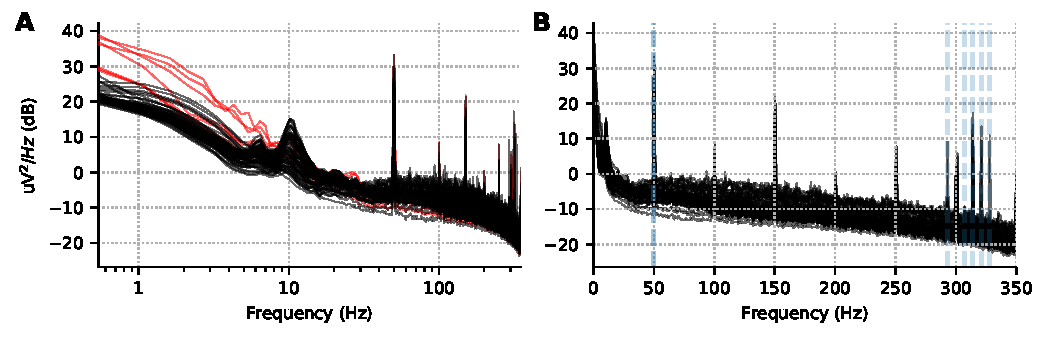
\includegraphics[width=\linewidth]{figures/psd.pdf}
        \vspace{-10pt}
        \caption[Power spectral density to mark bad channels and check filtering]{Power spectral density per channel for subject 10, run 02. (A) Log scale for the x axis accentuates low frequency drifts in the data. The red lines show the PSD for the bad channels marked manually and provided to us by~\citet{wakeman2015multi}. (B) The same data with a linear x-axis scale. Five peaks corresponding to HPI coils around 300 Hz are visible and marked in gray dotted lines alongside the power line frequency (50 Hz).}
        \label{fig:fig1_plot_psd}
\end{figure}

The power spectral density (PSD) estimates for all available data channels provide a convenient way to check for spectral artifacts and, in some cases, bad channels. MNE computes the PSD of raw data using the standard Welch's method~\citep{Welch67,percival1993spectral}, whereby the signal for each channel is analyzed over consecutive time segments, with eventually some overlap. Each segment is windowed and then the power of the discrete Fourier transform (DFT) coefficients is computed and averaged over all segments. By making the assumption that  each of these segments provides a realization of a stationary process, the averaging procedure produces an unbiased estimate of the PSD with reduced noise.

Starting from MNE version 0.14, we show channel-wise PSD plots rather than an average across channels, as this facilitates spotting outlier channels. In Figure~\ref{fig:fig1_plot_psd}, we show the PSD for the EEG channels in one run for one subject. We use windows of length 8192 samples (about 7.4\,s given the 1.1\,kHz sampling rate) with no overlap. Using a power of 2 for the length and no overlap accelerates computations. Using a logarithmic frequency-axis scaling for the PSD enables quality control by facilitating screening for bad channels. In fact, we found that some potentially bad channels (e.g., EEG024 in subject 14 for run 01) were omitted by the authors of \citep{wakeman2015multi}, although they are clearly visible in such plots. Concretely we see a few channels with strongly increased low-frequency power below 1 Hz. On the other hand, using a linear frequency-axis scaling, we can convince ourselves easily that the data is unfiltered, as it contains clear peaks from power line at harmonics of 50 Hz, as well as the five Head Position Indicator (HPI) coils used to monitor the head position of the subject, at frequencies of 293, 307, 314, 321, and 328\,Hz.

\emph{Alternatives} The same could have been achieved with the multitaper method~\citep{percival1993spectral, slepian1978prolate}, where the data is multiplied element-wise by orthogonal data tapers. However, this method can be an order of magnitude slower than the Welch method for long continuous recordings. The multitaper method is indeed recommended for short data segments. Here we are interested in the PSD for diagnostic purposes on the raw continuous data, and we therefore use the Welch method, a.k.a. averaged periodogram method.

\subsection{Temporal filtering}
\label{sec:group_study_temporal_filtering}

In this study, we focused on event-related brain signals below 40\,Hz. We low-pass filtered our data at a 40\,Hz cutoff frequency with 10 Hz transition band. Such a filter does not affect \ac{ERP} signals of interest, attenuates the line frequency of 50\,Hz and all HPI coil frequencies. It also limits the effects of temporal ringing thanks to a wide transition band. Because the low-pass was sufficiently low, we did not employ a notch filter separately. Note that such a choice of filters is not necessarily a good default for all studies of event-related brain responses, as ERFs or ERPs can contain rather high frequencies (see for example \citep{gotz-etal:15}).

When filtering, it is important to take into account the frequency response and impulse response of the filter. In MNE 0.16, the default filter will adapt the filter length and transition band size based on the cutoff frequencies, as done in the EEGLAB software~\citep{widmann2015digital,parks1987digital,ifeachor2002digital}\footnote{\url{https://martinos.org/mne/stable/auto_tutorials/plot_artifacts_correction_filtering.html}}. Although no default parameters will fit all analysis requirements, MNE chooses parameters that aim to achieve reasonable stop-band attenuation without excessive filter ringing. To illustrate this point, we compare filters across MNE versions using frequency response and impulse response plots in Figure~\ref{fig:fig2_filter}. The stop-band attenuation and transition bandwidth in Figure~\ref{fig:fig2_filter}A and Figure~\ref{fig:fig2_filter}B are less restricted in the newer versions, which results in less steep attenuation but also less temporal ringing in the impulse response (see Figures~\ref{fig:fig2_filter}C and D). It can be seen that the previous default parameters gave rise to stronger filtering artifacts as indicated by higher impulse response amplitudes across the time window.

\begin{figure}[htb]
    \centering
    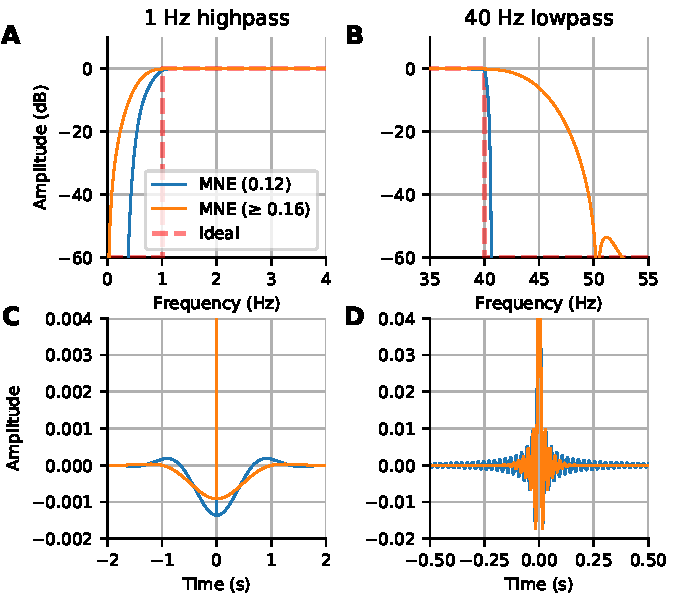
\includegraphics{figures/filters.pdf}
    \caption[Comparison of filters between new (0.16) and old (0.12) MNE versions.]{Comparison of filters between new (0.16) and old (0.12) MNE versions: (A) The frequency response of the highpass filter; (B) The frequency response of the lowpass filter; (C) The impulse response of the highpass filter; (D) The impulse response of the lowpass filter. The filters in MNE are now adaptive with trade-offs between frequency attenuation and time domain artifacts that by default adapt based on the chosen low-pass and high-pass frequencies.}
    \label{fig:fig2_filter}
\end{figure}

\emph{Alternatives and Caveats:} If the signal quality is satisfactory, filtering may not be necessary. In the context of this study, we decided to baseline correct our signals rather than high-pass filter them, keeping in mind the ongoing discussion in the community on this topic~\citep{tanner2015inappropriate,rousselet2012does,widmann2012filter,acunzo2012systematic,maess2016high}. Our choice will be motivated in Section~\ref{sec:baseline} on baseline correction.

\subsection{Marking bad segments and channels}

The next step in the pipeline is to remove bad data segments and bad channels. As data have been processed with Maxwell filter, there are no more bad \ac{MEG} channel at this stage. For the bad EEG channels, we use the ones provided by the original authors.

To remove bad data segments and bad epochs due to transient artifacts, it is possible in MNE to use the epochs plotter interactively, or to do it via scripting. Either way, the indices of all epochs that are removed from further analysis are logged in the \textit{drop log} attribute of the epochs objects (see online documentation of the Epochs class\footnote{\url{http://martinos.org/mne/stable/auto_tutorials/plot_epoching_and_averaging.html}}).

As we are building a reproducible pipeline, here we prefer the scripting route. In MNE, this can be achieved by removing trials whose peak-to-peak amplitude exceeds a certain rejection threshold. Even though this works reasonably well for single subject analysis, it would likely need to be tuned for individual subjects in group studies. Therefore, instead of specifying the thresholds manually, we learn it from the data using the \emph{autoreject} (global)~\citep{jas2017autoreject} algorithm. \emph{Autoreject} is an unsupervised algorithm which minimizes the cross-validation error, measured by the Frobenius norm between the average signal of the training set and the median signal of the validation set. \emph{Autoreject} not only removes trials containing transient jumps in isolated \ac{MEG} or \ac{EEG} channels, but also eyeblink artifacts affecting groups of channels in the frontal area. Since we are dealing with visual stimuli, it is preferable to remove the eyeblink trials altogether using the \ac{EOG} rejection threshold over the stimulus presentation interval rather than suppressing the artifact using a spatial filter such as \ac{ICA} or \ac{SSP}. Given the large number of trials at our disposal, we can afford to remove some without affecting the results very much.

For the purpose of group averaging, the bad \ac{EEG} channels were repaired by spherical spline interpolation~\citep{perrin1989spherical} so as to have the same set of channels for each subject.

\subsection{Independent Component Analysis (ICA)}
 
Bad channel or segment removal can correct for spatially and temporally isolated artifacts. However, it does not work well for systematic physiological artifacts that affect multiple sensors. For this purpose, \ac{ICA} is commonly used~\citep{jung1998extended}. \ac{ICA} is a blind source separation technique that maximizes the statistical independence between the components. While \ac{PCA} only requires orthogonal components, \ac{ICA} looks for independence for example by looking at higher statistical moments beyond (co)variance. In the context of MEG and EEG analysis, common physiological artifacts have skewed and peaky distributions, hence are easily captured by \ac{ICA} methods that look for non-Gaussian sources. \ac{ICA} is therefore popular for removing eye blinks and heart beats, which manifest themselves with prototypical spatial patterns on the sensor array.

In the present study, we use FastICA~\citep{hyvarinen1999fast} to decompose the signal into maximally independent components. We estimate the ICA decomposition on band-pass filtered (1\,Hz highpass with 1\,Hz transition band, 40\,Hz lowpass with 10\,Hz transition band) data that has been decimated. In practice, to improve the quality of ICA solution, high-pass filtering is often helpful as it can help to minimize violations of the stationarity assumption made by ICA. Likewise, it is recommended to exclude data segments containing environmental artifacts with amplitudes higher than the artifacts of interest. Finally, generous decimation can save computation time and memory without affecting the quality of the ICA solution, at least, when it comes to separating physiological artifacts from brain signals. Both measures can be implemented using the \code{reject} and \code{decim} parameters provided by the ICA fitting routine in MNE. Here we decimated the data by a factor of 11, and excluded time segments exceeding amplitude ranges of \SI{4000e-13} {\femto\tesla\per\centi\meter} and \SI{4e-12} {\femto\tesla} on the magnetometers and gradiometers, respectively.

The ICA component corresponding to ECG activity is then identified using \ac{CTPS}~\citep{dammers2008integration} using the default threshold of 0.8 on the Kuiper statistic. Pearson correlations are used to find EOG related components. As ICA is a linear model, the solution can be estimated on continuous \textit{raw} data and subsequently used to remove the bad components from the \textit{epochs} or \textit{evoked} data. 

\emph{Alternatives} MNE also implements CORRMAP~\citep{viola2009semi} which is particularly useful when no ECG or EOG channels are available. This approach uses pattern matching of ICA spatial components. Once templates have been manually defined for one subject, similar patterns can be found for the remaining subjects. If ICA is not an option, SSP projections provide a simple and fast alternative. Here, they can be computed from time segments contaminated by the EOG and ECG artifacts and commonly the first 1 to 2 components are projected out. In our experience, SSP is less precise in separating artifacts from brain components than ICA for the reasons mentioned above, yet, often good enough for a wide class of data analysis scenarios. For analysis of single EEG sensors, multivariate methods cannot be applied. Computing the residuals of a linear regression from the ECG sensor on the EEG is an option in this case.

\emph{Caveats.} Before blindly applying ICA, it is recommended to estimate the amount of contamination of the MEG and EEG signals. This can be easily achieved by detecting artifact events and epoching and averaging the data accordingly. If, for example, the amplitude range of the average ECG artifact is close to the amplitude range of the brain signals and only few events occur, chances are low to estimate clear cut ECG components using ICA. However, in this case the contamination by ECG is low and therefore no advanced artifact suppression is needed. Second, there is a trade-off between processing time and accuracy. For many analyses, mitigating the artifact contamination by a significant proportion is sufficient and methods like SSP are a reasonable choice. In certain decoding analyses, such preprocessing considerations may have little relevance if any for the final classification results. Indeed, the combination of supervised and multivariate decoding algorithms allows to extract the signals of interest directly in one step.

\subsection{Epoching}
\label{sec:epoching}
In event-related M/EEG studies, a trigger channel (in this data STI101) contains binary-coded trigger pulses to mark the onset/offset of events. These pulses can be automatically extracted from the data during analysis and the values on the trigger channel are mapped to the \textit{event IDs}. MNE offers the possibility to extract events when the signal in the trigger channel increases, decreases, or both. It also allows the construction of binary masks to facilitate selecting only the desired events. We masked out the higher order bits in the trigger channel when extracting the events as these corresponded to key presses. After extraction, events can be freely manipulated or created as necessary by the user, as they only require i) the sample number, and ii) some integer code relevant for the experiment or analysis.

As a next step, we extracted segments of data from the continuous recording around these events and stored them as single trials, which are also called epochs, in MNE. The \code{Epochs} object can store data for multiple events and the user can select a subset of these as \code{epochs[event\_id]}\footnote{\url{http://martinos.org/mne/stable/auto_tutorials/plot_epoching_and_averaging.html}}. Moreover, MNE offers the possibility for the user to define a hierarchy of events by using tags (similar in flavor to hierarchical event descriptors by~\cite{bigdely2013hierarchical}). This is done using \code{event\_id} which is a dictionary of key-value pairs with keys being the tags separated by a forward slash (\code{\//}) and values being the trigger codes\footnote{\url{http://martinos.org/mne/stable/auto_tutorials/plot_object_epochs.html}}. For the paradigm used in this study we used:
      \begin{lstlisting}[]
      events_id = {
      'face/famous/first': 5,
      'face/famous/immediate': 6,
      'face/famous/long': 7,
      'face/unfamiliar/first': 13,
      'face/unfamiliar/immediate': 14,
      'face/unfamiliar/long': 15,
      'scrambled/first': 17,
      'scrambled/immediate': 18,
      'scrambled/long': 19,
      }
      \end{lstlisting}
At the highest level of hierarchy are `face' and `scrambled'. A `face' can be `famous' or `unfamiliar'. And a famous face can be `first', `immediate' or `long' (This distinction between the three categories of famous faces was not used in our analysis). Later on, accessing all the epochs related to the `face' condition is straightforward, as one only needs to use \code{epochs['face']} and MNE internally pools all the sub-conditions together.
Finally, the epochs were constructed starting 200\,ms before stimulus onset and ending 2900\,ms after (the earliest possible time of the next stimulus onset).

% When constructing the epochs, we decimate the data by a factor of two by selecting every other sample in the data.
%       \begin{lstlisting}
%       from mne import Epochs
%       epochs = Epochs(raw, tmin=-0.5, tmax=0.5)
%       \end{lstlisting}
   
\subsection{Baseline correction}
\label{sec:baseline}

\begin{figure}[t]
  \centering
  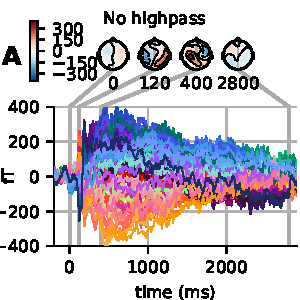
\includegraphics[width=0.31\linewidth]{figures/FanningA.pdf}
  \hspace{0.5em}
  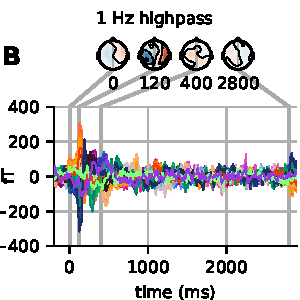
\includegraphics[width=0.31\linewidth]{figures/FanningB.pdf}
  \hspace{0.5em}
  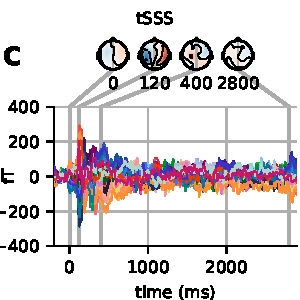
\includegraphics[width=0.31\linewidth]{figures/FanningC.pdf}
\caption[Comparison of highpass filtering and tSSS on evoked response.]{(A) Evoked response in magnetometers for subject 3 with baseline correction. Note how signals tend toward the baseline late in the epochs (where the rightmost time point, 2.9 sec, is the earliest possible start time for the next stimulus). (B) The highpass filtered version of the signal and (C) the signal processed with temporal SSS (tSSS). Both reduce the magnitude of the slow and late sustained responses shown in (A).}
\label{fig:fanning}
\end{figure}
  
It is common practice to use baseline correction so that any constant offsets in the baseline are removed. High-pass filtering achieves similar results by eliminating the low-frequency components in the data. However, when using baseline correction, the low frequency drifts present in the data are not attenuated. Thus it is useful to examine long time-courses of the data, if possible, to determine if low-frequency drifts are present. The difference between the two approaches can be seen in Figure~\ref{fig:fanning}. The evoked responses in the figure are across-trial averages for the famous face condition. If a maximum time of approximately one second were used, a simple baseline correction would appear to produce an undesired \textit{``fanning"} in the later responses. Indeed one can observe in Figure~\ref{fig:fanning}A that at one second post-stimulus, the channels still significantly deviate from zero. However, by extending the time window much longer (here to 2.9 seconds) we can see that the signals do mostly return to the baseline level.

\emph{Caveats and Alternatives} With highpass filter at 1\,Hz (and 1 Hz transition band), the signal returns to the baseline level much sooner. Note also the similarities between Figures~\ref{fig:fanning}B and~\ref{fig:fanning}C, illustrating how using temporal version of the SSS algorithm (tSSS) acts implicitly as a high-pass filter. For tSSS, we use a buffer size of length 1\,s and a correlation limit of 0.95 to reject overlapping inner/outer signals. However, these high-passing effects come at the expense of distorting the sustained responses. We will thus focus on analyses that utilize the baseline-corrected data here.
